\documentclass[10pt,spanish,a4paper,openany,notitlepage]{article}
%-------------------------------------Paquetes-----------------------------------------------------------------------
\usepackage[spanish,es-tabla]{babel}  	% Traduce los textos a castellano
\usepackage[utf8]{inputenc}	% Permite escribir directamente áéíóúñ
\usepackage{t1enc}            	% Agrega caracteres extendidos al font
\usepackage{amsmath} 		%Permite imprimir mas opcciones matematicas
\usepackage{graphicx}		%Permite agregar imagenes al informe
\usepackage{multicol}  		%Permite dividir el texto en varias columnas
\usepackage{float} 		%Permite utilizar H para colocar las imagenes en un lugar especifico 
\usepackage{units}
\usepackage{circuitikz}
\usepackage{caption}
\usepackage{subcaption}
\usepackage{sidecap}
\usepackage{mathtools}
\usepackage{multirow} % Paquete para dividir las tablas en subtablas
\usepackage{booktabs} %estos 2 sirven para achicar la tabla
\usepackage{tabulary}
\usepackage{fancyhdr} % encabezado
\usepackage{textcomp} % para usar ° con el comando \textdegree
\usepackage{anysize}		%Permite modificar los margenes del documento
\usepackage{abstract} % paquete para el resumen del articulo
 
%---------------------------------------Configuraciones de pagina----------------------------------------------
\marginsize{2.5cm}{2.5cm}{1cm}{1cm}

\pagestyle{fancy}
\fancyhf{}
\lhead{
66.25 - \textsc{Dispositivos Semiconductores}\\ 
2\textsuperscript{do} Cuatrimestre de 2014
}
\rhead{
\includegraphics[width=3cm]{imagenes/FIUBA_ALTA.jpg}}
\rfoot{Página \thepage}

%---------------------------------------Definiciones propias---------------------------------------------------------
\newcommand{\oiint}{\displaystyle\bigcirc\!\!\!\!\!\!\!\!\int\!\!\!\!\!\int} %Integral doble cerrada

\DeclarePairedDelimiter\abs{\lvert}{\rvert}%
\DeclarePairedDelimiter\norm{\lVert}{\rVert}%
% Swap the definition of \abs* and \norm*, so that \abs
% and \norm resizes the size of the brackets, and the 
% starred version does not.
\makeatletter
\let\oldabs\abs
\def\abs{\@ifstar{\oldabs}{\oldabs*}}
%
\let\oldnorm\norm
\def\norm{\@ifstar{\oldnorm}{\oldnorm*}}
\makeatother
%--------------------------------------------------------------------------------------------------------------------------------


\makeatletter
\let\ps@plain\ps@fancy 
\makeatother

% lo siguiente es para borrar el titulo del resumen y que no ocupe espacio:
 \AtBeginDocument{%
 \renewcommand{\abstractname}{}%
 }
\renewcommand{\absnamepos}{empty} % originally center
 

\begin{document}
\title{\textbf{TP N\textdegree2: Curvas características del transistor TBJ BC548C}}
\author{
  Accifonte, Franco - 93799\\
  \texttt{franco.accifonte@gmail.com}  
  \and
  Iturria, Germán  - 86270 \\
  \texttt{german.iturria@gmail.com}
  \and
   Vázquez, Matías - 91523\\
  \texttt{mfvazquez@gmail.com}
}
\date{30 de octubre de 2014}
\maketitle

\begin{abstract} %Resumen
\emph{En el siguiente trabajo se analizan las principales características de polarización y frecuencias medias de transistores TBJ tipo NPN. Estudiando las curvas de transferencia y de salida, obtenidas en mediciones, se consiguen los parámetros característicos y se calculan los parámetros de pequeña señal. Finalmente se realiza un modelo básico de Spice con los parámetros calculados y se presentan simulaciones para contrastar con las mediciones.}
\end{abstract}

\section{Desarrollo}

A continuación se detalla el desarrollo del trabajo realizado, tanto la realización de las simulaciones mediantes \emph{Spice}, como las mediciones realizadas.

\subsection{Simulación de transistores BC548C}

En primera instancia se obtuvieron con \emph{LTSPICE} las curvas de transferencia, la ganancia de corriente entre base y colector y las curvas de salida  propias al transistor. Usando las bibliotecas  
 \texttt{PHIL\_BJT} y \texttt{SIEMENS} proporcionadas por la cátedra.

\subsubsection{Curva de transferencia}

Se simuló $I_C$ vs. $V_{BE}$ para $V_{CE} = 1,25 \unit{V}$ para ambas bibliotecas. Se varió la tensión $V_{BE}$ entre $0\unit{V}$ y $0,9\unit{V}$ con pasos de $0,01\unit{V}$, utilizando el circuito simulado en la figura \ref{circuito:simulacion_transferencia}.

\begin{figure}[H]
\centering
\begin{circuitikz}[american]\shorthandoff{>}
\draw 
(1.5,2) node[npn](npn){BC548C}
(0,0.5)  node[ground]{} to [V, l=$V_{BE}$] (0,2) -- (npn.base)
(1.5,0.5)node[ground]{} -- (npn.emitter) 
(3,0.5)  node[ground]{} to [V, l_= $V_{CE}$] (3,2.77) -- (npn.collector)
;\end{circuitikz}
\caption{Circuito utilizado para la obtención de las curvas de transferencia.}
\label{circuito:simulacion_transferencia}
\end{figure}

\subsubsection{Ganancia de corriente entre base y colector}

Para ambas bibliotecas se simuló el circuito de la figura \ref{circuito:simulacion_ganancia_salida} bajo las condiciones de medición del multímetro que se utilizará en las mediciones. Estas son $I_B = 10\unit{\mu A}$ y $V_{CE} = 2,8\unit{V}$. Se obtuvo el parámetro \texttt{BETADC} del \texttt{Simulation Output File}.

\begin{figure}[H]
\centering
\begin{circuitikz}[american]\shorthandoff{>}
\draw 
(1.5,2) node[npn](npn){BC548C}
(0,0.5)  node[ground]{} to [I, l=$I_{B}$] (0,2) -- (npn.base)
(1.5,0.5)node[ground]{} -- (npn.emitter) 
(3,0.5)  node[ground]{} to [V, l_= $V_{CE}$] (3,2.77) -- (npn.collector)
;\end{circuitikz}
\caption{Circuito utilizado para la obtención de las curvas de salida y de la ganancia de corriente.}
\label{circuito:simulacion_ganancia_salida}
\end{figure}

Se obtuvieron los siguientes valores:

\begin{itemize}
\item{\texttt{PHIL\_BJT}}: $h_{FE} = 460$
\item{\texttt{SIEMENS}}: $h_{FE} = 432$
\end{itemize}

\subsubsection{Curva de salida}

Se simuló $I_C$ vs. $V_{CE}$ para $I_{B} = cte$ para ambas bibliotecas. Se varió la tensión $V_{CE}$ entre $0\unit{V}$ y $5\unit{V}$ con pasos de $0,01\unit{V}$, utilizando el circuito simulado en la figura \ref{circuito:simulacion_ganancia_salida}.

La corriente $I_B$ se determinó mediante la ecuación \ref{eq:I_B} para cada valor de $I_C$ deseado, utilizando el parámetro $h_{FE}$ correspondiente al transistor de cada biblioteca. 

\begin{equation}
I_B = \frac{I_C}{h_{FE}}
\label{eq:I_B}
\end{equation}

A continuación se listan los valores de $I_B$ utlizados.

\begin{itemize}
\item{\texttt{PHIL\_BJT} con $h_{FE} = 460$}
\begin{itemize}
\item{$I_C = 5 \unit{mA}$}: $I_B = 10,9\unit{\mu A}$
\item{$I_C = 25 \unit{mA}$}: $I_B = 54,3\unit{\mu A}$
\end{itemize}
\item{\texttt{SIEMENS} con $h_{FE} = 432$}
\begin{itemize}
\item{$I_C = 5 \unit{mA}$}: $I_B = 11,6\unit{\mu A}$
\item{$I_C = 25 \unit{mA}$}: $I_B = 57,9\unit{\mu A}$
\end{itemize}
\end{itemize}

\subsection{Obtención de parámetros de las hojas de datos}

\subsection{Obtención de las curvas de forma experimental}

Se obtuvieron las curvas de tres transistores \textbf{TBJ BC548C} distintos utilizando una placa experimental, un regulador de tensión \textbf{LM317} y un \textbf{LM7805}, un potenciómetro lineal de $20\unit{k\Omega}$ y resistencias de valores apropiados para cada medición.
También se midió para cada transistor el valor de $h_{FE}$ utilizando un muletillero con esta función.

\subsubsection{Curva de transferencia}

Para obtener la curva $i_C$ vs $v_{BE}$ se utilizó el banco de mediciones presentado en la figura \ref{circuito:medicion_transferencia}. El regulador de tensión \textbf{LM317} fija la tensión $V_{CE}=1,25\unit{V}$ y el regulador de tensión \textbf{LM7805} provee una alimentación constante de $5\unit{V}$. El potenciómetro utilizado es de $20 \unit{k\Omega}$.

\begin{figure}[H] %[h] para here [b] para bottom [t] para top [H]+float para aqui si o si
\begin{center}
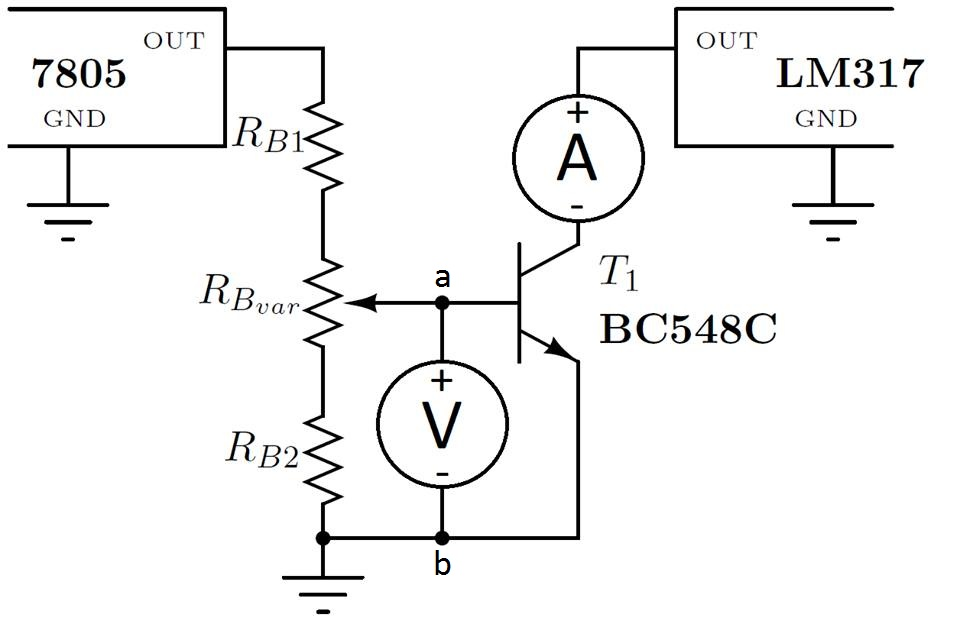
\includegraphics[scale=0.3]{./imagenes/ic_vbe.jpg}
\caption{Circuito para la medición de la curva de transferencia $I_C$ vs. $V_{BE}$}
 \label{circuito:medicion_transferencia}
\end{center}
\end{figure}

Para la obtención de las resistencias $R_{B1}$ y $R_{B2}$ se partió planteando el rango de la corriente $I_C$ deseado y suponiendo $h_{FE} = 200$ se obtuvo el rango de $I_B$.

\[ \displaystyle 0 \unit{mA} \leq I_C \leq 50\unit{mA} \ \ \ \ \ \Longrightarrow \ \ \ \ \  0 \unit{\mu A} \leq I_B \leq 250 \unit{\mu A} \]

Luego se obtuvo el equivalente de Thévenin entre los terminales $a$ y $b$. Para simplificar las ecuaciones se utilizó $R_1 = R_{B1} + R_{B1_{var}}$ y $R_2 = R_{B2} + R_{B2_{var}}$ con $R_{B_{var}} = R_{B1_{var}} + R_{B2_{var}} = 20 \unit{k\Omega}$. Siendo $R_{B_{var}}$ el potenciometro de $20 \unit{k\Omega}$.

\[ \displaystyle V_{TH} = V_{DD} \frac{R_1}{R_1 + R_2}\ \ \ \ \ \ \ \ \ \ R_{TH} = \frac{R_1\ R_2}{R_1 + R_2}\]

Siendo $V_{DD}$ la salida del regulador de tensión \textbf{LM7805}. 

Del circuito mostrado en la figura \ref{circuito:medicion_transferencia} obtenemos la ecuación \ref{eq:I_B}

\begin{equation}
\displaystyle I_B = \frac{V_{TH} - V_{BE_{ON}}}{R_{TH}}
\label{eq:I_B}
\end{equation}

Reemplazando la ecuación \ref{eq:I_B} en el rango de valores deseado.

Para el mínimo valor de $I_B$:

\[ \displaystyle \frac{V_{TH} - V_{BE_{ON}}}{R_{TH}} \geq 0 \unit{\mu A} \]

Entonces:

\begin{equation}
V_{TH} \geq V_{BE_{ON}}
\label{eq:Vth_baja}
\end{equation}

Para el máximo valor de $I_B$:

\begin{equation}
\frac{V_{TH} - V_{BE_{ON}}}{R_{TH}} \leq 250 \unit{\mu A}
\label{eq:Vth_alta}
\end{equation}

Con las inecuaciones \ref{eq:Vth_baja} y \ref{eq:Vth_alta} se buscaron valores de $R_{B1}$ y $R_{B2}$ que las cumplam. Teniendo en cuenta que para cada inecuacion los valores de $V_{TH}$ y $R_{TH}$ son distintos ya que dependen de $R_1$ y $R_2$ que varían por estar conectados a un potenciómentro y $0,5 \unit{V} \leq V_{BE_{ON}} \leq 0,7 \unit{V}$.\\

Se propusieron los siguientes valores $R_{B1} = 5\unit{k\Omega}$ y $R_{B2} = 25\unit{k\Omega}$:

\begin{itemize}
\item{Para $I_B \geq 0 \unit{\mu A}$}: $V_{BE_{ON}} = 0,5 \unit{V}$, $R_1 = R_{B1} = 5 \unit{k\Omega}$ y $R_2 = R_{B2} + 20\unit{k\Omega} = 45 \unit{k\Omega}$

Obteniendo los siguientes valores para el equivalente de Thévenin:

\[ \displaystyle V_{TH} =  0,5 \unit{V} \geq 0,5 \unit{V} = V_{BE_{ON}}\]

\item{Para $I_B \leq 250 \unit{\mu A}$}: $V_{BE_{ON}} = 0,7 \unit{V}$, $R_1 = R_{B1}+ 20\unit{k\Omega} = 25 \unit{k\Omega}$ y $R_2 = R_{B2} = 25 \unit{k\Omega}$

\[ \displaystyle V_{TH} =  2,5 \unit{V} \ \ \ \ \ \ \ \ \ \  R_{TH} = 12,5 \unit{k\Omega}\]

\[ \displaystyle \frac{V_{TH} - V_{BE_{ON}}}{R_{TH}} = \frac{2,5 \unit{V} - 0,7 \unit{V}}{12,5 \unit{k\Omega}} = 144 \unit{\mu A} \leq 250 \unit{\mu A} \]

Entonces el valor maximo medido de $I_C$ será: $I_{C_{MAX}} = I_B\ h_{FE} = 144 \unit{\mu A}\ 200 = 28,8 \unit{mA}$

\end{itemize}

Como se ve los valores $R_{B1}$ y $R_{B2}$ elegidos cumplen las condiciones esperadas.

\subsubsection{Ganancia de corriente entre base y colector}

Para obtener $h_{FE}$ se utilizó un multímetro que realiza la medición bajo las condiciones $I_B = 10 \unit{\mu A}$ y $V_{CE} = 2,8 \unit{V}$

Se obtuvieron los siguientes valores para cada transistor:

\begin{itemize}
\item{Transistor 1:} $h_{FE} = 361$
\item{Transistor 2:} $h_{FE} = 326$
\item{Transistor 3:} $h_{FE} = 253$
\end{itemize}

\subsubsection{Curva de salida}

Para obtener la curva $i_C$ vs $v_{CE}$ se utilizó el banco de mediciones presentado en la figura \ref{circuito:medicion_salida}.El regulador de tensión \textbf{LM7805} provee una alimentación constante de $5\unit{V}$. El potenciómetro utilizado es de $20 \unit{k\Omega}$.

\begin{figure}[H] %[h] para here [b] para bottom [t] para top [H]+float para aqui si o si
\begin{center}
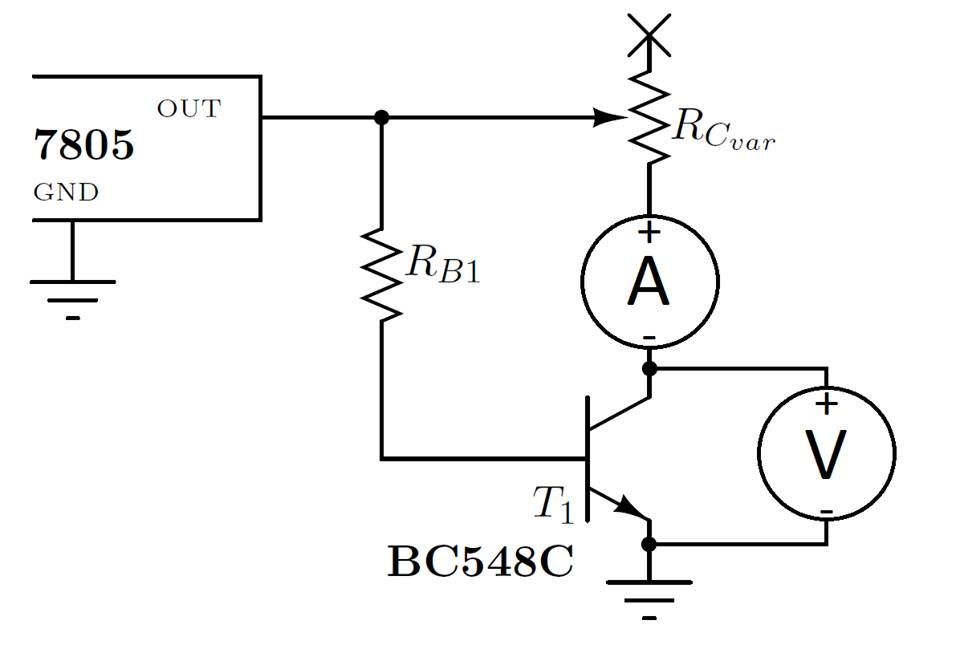
\includegraphics[scale=0.2]{./imagenes/ic_vce.jpg}
\caption{Circuito para la medición de la curva de salida $I_C$ vs. $V_{CE}$}
 \label{circuito:medicion_salida}
\end{center}
\end{figure}

Para la obtención de la resistencia $R_{B1}$ planteamos la ecuación obtenida del circuito mostrado en la figura \ref{circuito:medicion_salida}:

\[ \displaystyle R_{B1} = \frac{V_{DD} - V_{BE_{ON}}}{I_B} \]


Y teniendo en cuenta que $I_B = \frac{I_C}{h_{fe}}$ se llegó a la ecuación \ref{eq:RB1}

\begin{equation}
R_{B1} = \frac{(V_{DD} - V_{BE_{ON}}) h_{FE}}{I_C}
\label{eq:RB1}
\end{equation}

Siendo $V_{DD} = 5 \unit{V}$ la salida del regulador de tensión  \textbf{LM7805} y $V_{BE_{ON}} = 0,7 \unit{V}$

A continuación listamos los valores de $R_{B1}$ para cada transistor y para cada $I_C$:

\begin{itemize}

\item{Transistor 1:} $h_{FE} = 361$

\begin{itemize}
\item{Para $I_C = 5 \unit{mA}$}: $R_{B1} \approx 310 \unit{k\Omega}$
\item{Para $I_C = 25 \unit{mA}$}: $R_{B1} \approx  62\unit{k\Omega}$
\end{itemize}

\item{Transistor 2:} $h_{FE} = 326$

\begin{itemize}
\item{Para $I_C = 5 \unit{mA}$}: $R_{B1} \approx  280\unit{k\Omega}$
\item{Para $I_C = 25 \unit{mA}$}: $R_{B1} \approx  56\unit{k\Omega}$
\end{itemize}

\item{Transistor 3:} $h_{FE} = 253$

\begin{itemize}
\item{Para $I_C = 5 \unit{mA}$}: $R_{B1} \approx  217\unit{k\Omega}$
\item{Para $I_C = 25 \unit{mA}$}: $R_{B1} \approx  43\unit{k\Omega}$
\end{itemize}

\end{itemize}

\subsection{Obtención de parámetros a partir de las mediciones}

\subsubsection{Parámetros característicos}

\subsubsection{Parámetros de pequeña señal}



\subsection{Simulación del modelo modificado}

Se diseñó un modelo modificado basado en el modelo de \emph{Spice} del TBJ NPN genérico ajustado a los parámetros característicos del Transistor 1. Realizamos las mismas simulaciones que para las bibliotecas \texttt{PHIL\_BJT} y \texttt{SIEMENS} incluyendo la siguiente directiva:\\

\texttt{.MODEL MiModelo NPN (BF=361 IS=106.239f VAF=86.67009)}\\

Para la simulación de la ganancia de corriente entre base y colector se obtuvo $h_{FE} = 370$

\section{Análisis y comparación de los resultados}

\subsection{Curvas obtenidas}

\subsection{Comparación de los resultados}

\section{Conclusiones}

\end{document}